\documentclass[english,onecolumn]{article}
\usepackage{graphicx}
%\usepackage{txfonts}
\usepackage{epstopdf}
\usepackage{amsmath}
%\usepackage{float}

\begin{document}

\author{Rasmus Skriver}
\title{Report on the error function}
\author{Rasmus Skriver: 201507256}

\maketitle

The error function, also know as the Gauss error function, is a mathematical function gicen by 

\begin{equation}
\textrm{erf}(x)=\frac{1}{\sqrt{\pi}} \int _{-x} ^{x} e^{-t^{2}}\,dt.
\end{equation}

It usually occurs in probability, statistics, and partial differential equations 
describing diffusion.

It can be seen plotted in figure \ref{fig:error}.

\begin{figure}[h]
\centering
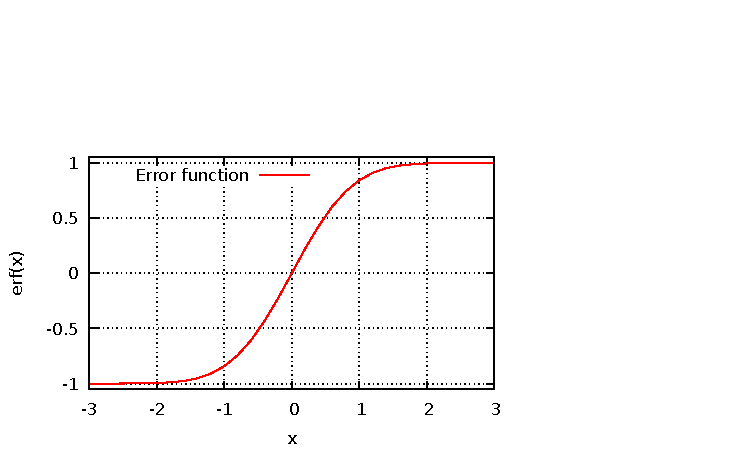
\includegraphics{plot.pdf}
\caption{A plot of the error function on the interval [-3,3].}
\label{fig:error}
\end{figure}

\end{document}
